\section{Proposed Approach} % (fold)
\label{sec:own_approach}

The \crowdre{} dataset is available in form of a MySQL database dump, but the tables can also be downloaded separated into several \textit{.csv} files \cite{crowdre_dataset}. For our research, we were only interested in the pure requirement sentences (without any ratings, or user characterization added to the data). We therefore reconstructed the sentences from the \textit{requirements.csv} file, which is included in the downloaded data.

To have some measure to evaluate the proposed approach we need a labeling at the dataset that we can use to rate how good the topic modeling worked. At first we checked if we can use the user defined tags as soft labeling for the requirements. Unfortunately most of them are only matched once (Total tags: 2116, tags that only occur once: 1562). Additionally we evaluated the most common used tags and the coverage\footnote{specific number of tags covering a significant amount of requirements} of the requirements.

\begin{figure}[ht]
  \centering
    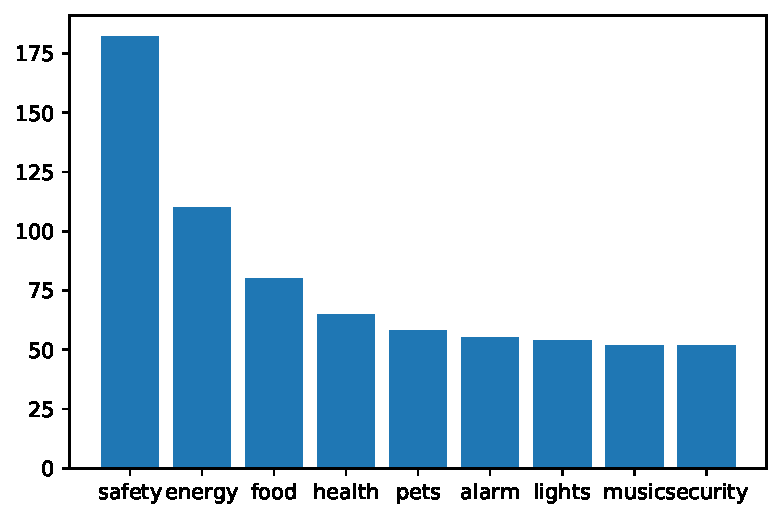
\includegraphics[width=0.8\textwidth]{screenshots/tag_analysis.pdf}
    \caption{Tag occurrence and coverage of the requirements}
    \label{fig:tag_analysis}
\end{figure}
\FloatBarrier

In \autoref{fig:tag_analysis} the coverage of requirements by the given tags is shown. The fact that about $\frac{1562}{2116}\approx73.8\,\%$ of the tags only occur once leads to a small coverage of requirements by the given tags. The variety of tags that may be assigned to the same topic is very high and the low coverage of requirements with the top 9 tags makes the tags not suitable for the soft labeling. 

Another approach to get a labeling for the evaluation was to check the domains that were assigned to the requirements. The domains are separated into five groups: Health, Energy, Entertainment, Safety and Other. For the \grqq{}Other\grqq{} there are again user defined specific domains, but we focus on the five top level domains for our labeling.

\subsection{NLP Preprocessing Pipeline} % (fold)
\label{sub:own_pipeline}

\begin{figure}[ht]
  \centering
    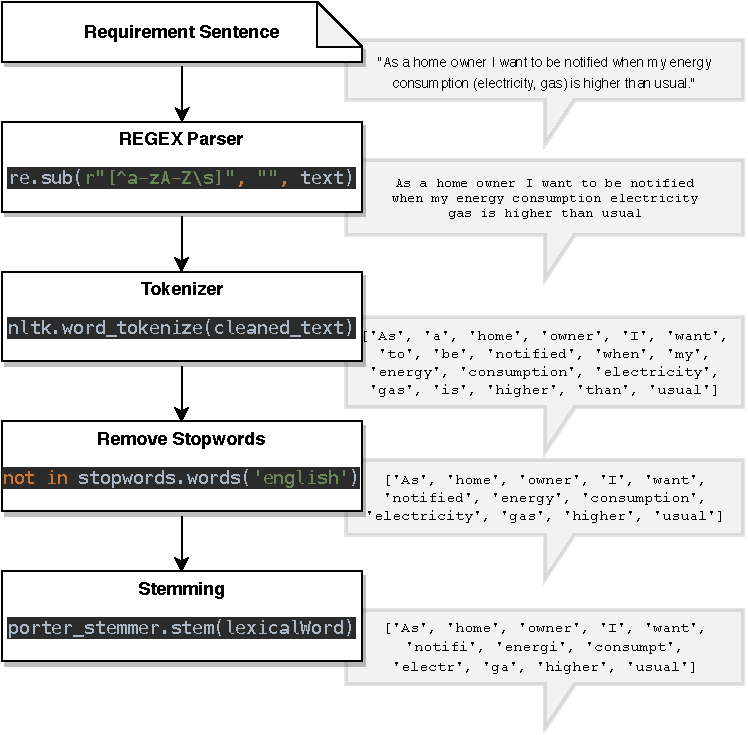
\includegraphics[width=\textwidth]{figures/NLP Pipeline.pdf}
    \caption{Processing an exemplary requirement sentence through our NLP Preprocessing Pipeline.}
    \label{fig:nlp_pipeline}
\end{figure}

As initially described in \autoref{sec:nlp} we preprocessed our requirement documents using an NLP pipeline as shown in \autoref{fig:nlp_pipeline}. Implementing our solution in Python and following the common practice as suggested in \cite{ferrari_natural_2018}, we made use of the NLTK library \cite{nltk_library} to perform the NLP techniques needed for our analysis. As some of the requirements sentences contains special characters, some initial data cleansing was necessary, to remove these special characters (i.e. spaces, dots, apostrophes, slashes) as they would have otherwise been ranked in the later used bag of words. We used regular expressions as provided by the Python standard library in order to do so. For the tokenization, the stop-word-removal and the stemming we used the functions provided by the NLTK API.
% subsection preprocessing (end)
\subsection{LDA Approach} % (fold)
\label{sub:own_lda}

After we developed our pre-processing pipeline for the dataset and some basic analysis on the data we have we decided to use the LDA for a first topic modelling. The LDA approach serves as reference for the result we wanted to obtain by the neural network to have a result for evaluating.


For our LDA approach we used our pre-processed requirements. To apply the LDA we transformed the data in the following way. We created a matrix where each row represents one of the 2966 requirements. the columns are the single words of the requirements. But as the LDA needs a numerical representation of the words we first applied a bag-of-words to the single requirements. As the results were not sufficient we decided to calculate the TF-IDF to get weights for the single words. After these steps we had a prepared matrix that holds the data that now can be used for the LDA.

\begin{figure}[bht]
    \subfigure[LDA Plot with colors to topics\label{fig:lda-tf-idf-topics}]{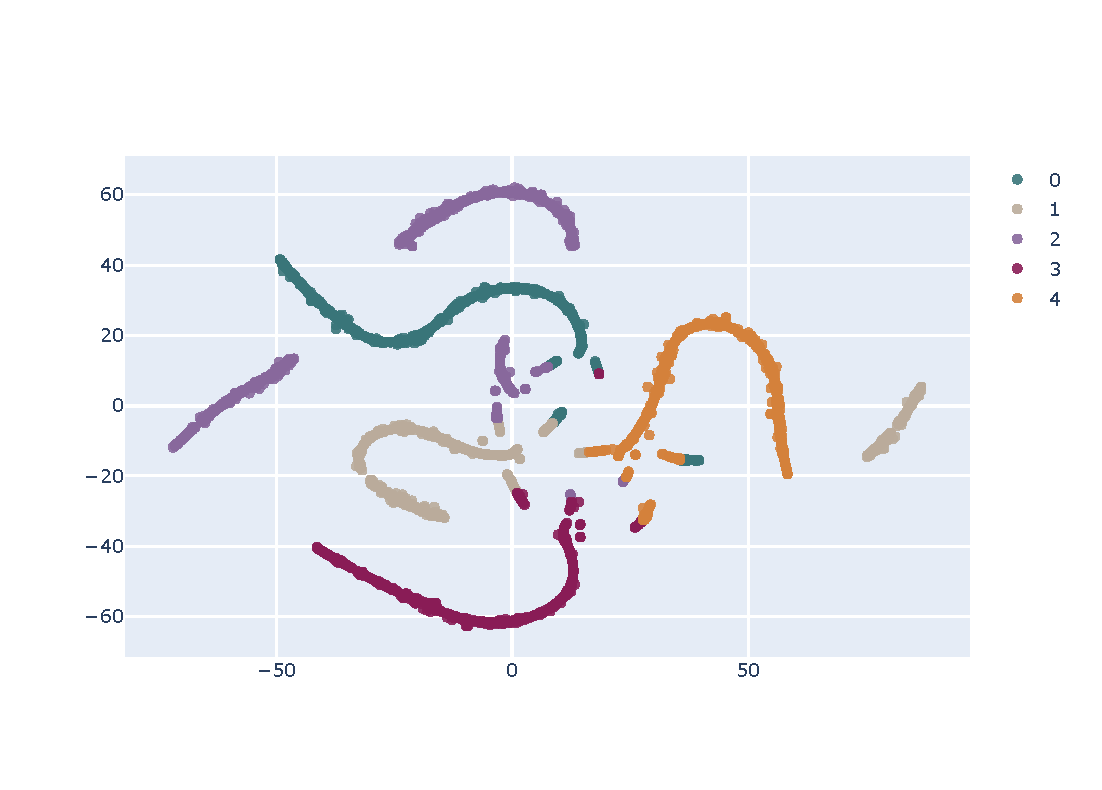
\includegraphics[width=0.49\textwidth]{screenshots/lda-tf-idf.pdf}}
    \subfigure[LDA Plot with colors for domains\label{fig:lda-tf-idf-domains}]{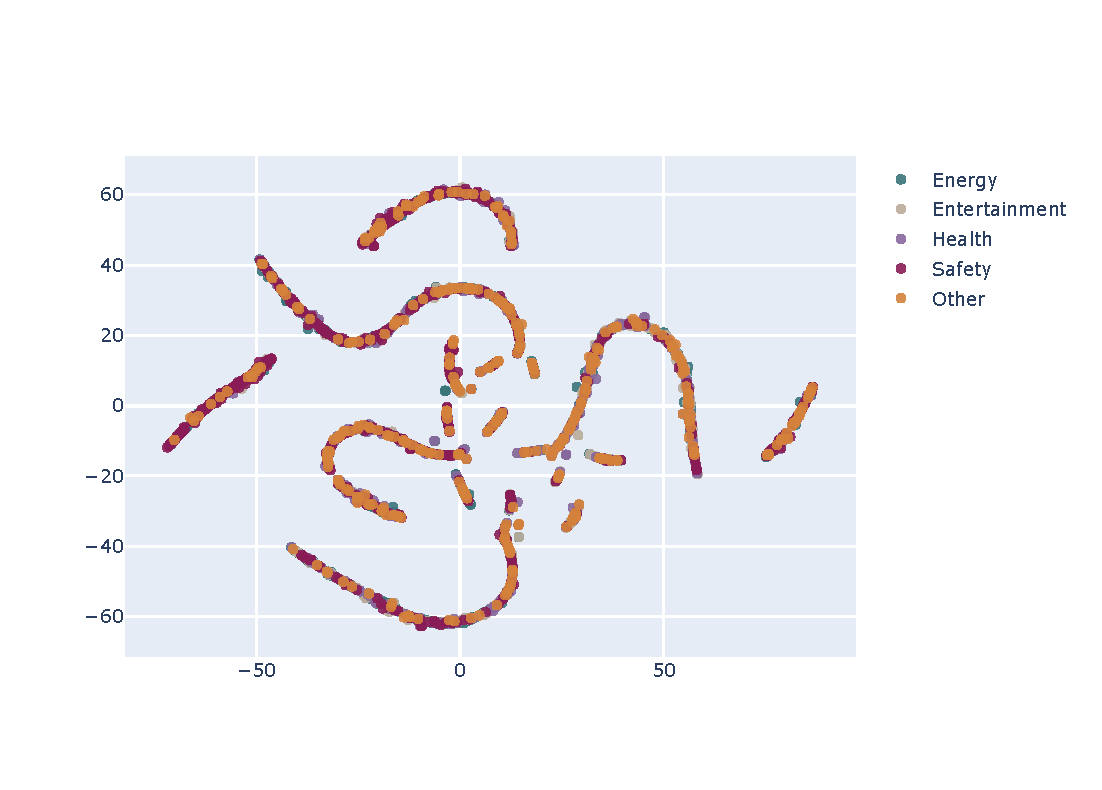
\includegraphics[width=0.49\textwidth]{screenshots/lda-domains.pdf}}
    \caption{LDA Result with TF-IDF (plotted with t-SNE)} \label{fig:lda-tf-idf}
\end{figure}
\FloatBarrier

In \autoref{fig:lda-tf-idf} we can see the two dimensional representation of the results of the LDA. The reduction of the dimensions is performed by t-SNE which tries to preserve the most differing dimensions. In \autoref{fig:lda-tf-idf-topics} the colors are mapped to the found topics which leads to separable clusters. But if we look for the expected mapping to the domains in \autoref{fig:lda-tf-idf-domains} we can see that the found cluster doesn't represent the expected clusters that where defined by the domains.
\subsection{Word Embeddings}
In order for our approach to also respect the semantic regularities of the requirements sentences, it is not enough to rely on the clusters generated by the LDA, as mentioned in \autoref{sub:back_word_embeddings}. We therefore create word embeddings for the corpus of requirements sentences we derived from the \crowdre{} dataset, using the techniques described earlier.

\subsubsection{word2vec} % (fold)
\label{sub:own_word2vec}
As shown in \autoref{fig:w2v-pipeline}, we use the word2vec implementation of the \textit{gensim} library to train language models on both word2vec architectures, with and without pre-processing the requirements through our NLP pipeline before. The outcome are 50-dimensional word vectors which form the basis for our clustering. With our dataset being relatively small, the created vectors may not capture all the semantic regularities, though\,\cite{mikolov_distributed_2013}. We therefore also use the word vectors Mikolov et al. created in order to measure the performance of their word2vec architectures, in 2013\,\cite{mikolov_efficient_2013}. Instead of the approximately 50.000 words in the \crowdre{} dataset, they trained their language model on the Google News dataset with 100 billion words. We thus expect the quality of these word vectors to be much higher and as such to positively affect our later results.
\begin{figure}[ht]
  \begin{center}
    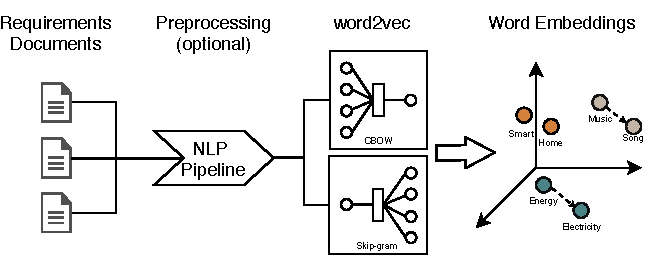
\includegraphics[width=0.9\textwidth]{figures/word2vec_pipeline.pdf}
    \caption{Training a language model on our requirements corpus to create word embeddings using word2vec.}
    \label{fig:w2v-pipeline}
  \end{center}
\end{figure}
\FloatBarrier

With the word embeddings, every word in the \crowdre{} dataset can be represented as a multidimensional vector. We could now create a matrix, representing the whole vocabulary in word vectors, as shown in \autoref{fig:embeddings_matrices} (1). Applying K-Means to the matrix, we would then cluster all the words in the dataset into topics. To cluster the dataset on a sentence level instead, we perform the following four steps:

\begin{enumerate}
\item We create a matrix for every sentence in the corpus, by replacing each word with its vector representation (see \autoref{fig:embeddings_matrices} (2)). The x-dimension of the matrix depends on the length of the sentence, the y-dimension is determined by the length of the word vectors. Using our own 50-dimensional word vectors and e.g. a sentence with 10 words, the shape of the matrix will be $10\times50$.
\item As the sentences in the dataset are of different lengths, the x-dimensions of the matrices are different, too. We use Principal Component Analysis (PCA)\,\cite{wold_principal_1987} to reduce the different x-dimensions to length of the shortest sentence (or the lowest x-dimension respectively).
\item We combine all these sentence matrices in a single matrix $T$, which is a 3-dimensional matrix of the form $T\in\mathbb{R}^{n \times d \times s}$, where $n$ is the total number of sentences, $d$ is the dimension of the word vectors and $s$ is the length of the shortest sentence in the dataset.
\item To cluster our results with K-Means, we need to further transform this matrix into two-dimensional space. We do this by reshaping the matrix $T$ to a matrix $T'$ with $T' \in \mathbb{R}^{n \times d * s}$\footnote{This is done using the reshape-function of the numpy array implementation: \url{https://www.w3resource.com/numpy/manipulation/reshape.php}}.
\end{enumerate}
Finally, we cluster the sentences by applying K-Means to the resulting matrix $T'$.

\begin{figure}[ht]
  \begin{center}
    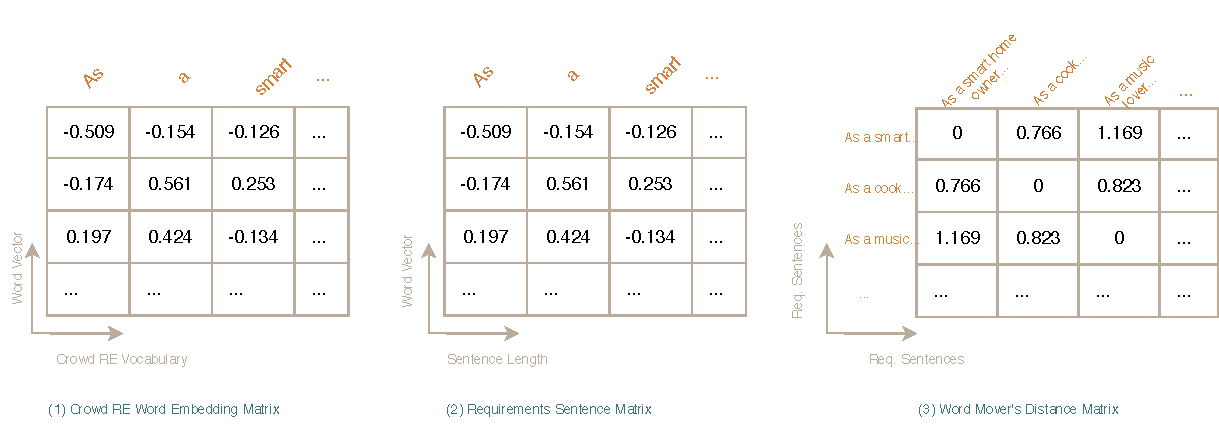
\includegraphics[width=\textwidth]{figures/embedding_matrices.pdf}
    \caption{Representing the \crowdre{} dataset using word embeddings.}
    \label{fig:embeddings_matrices}
  \end{center}
\end{figure}
\subsubsection{Word Mover's Distance} % (fold)
\label{sub:own_wmd}
As mentioned in \autoref{sub:word_movers_distance}, the document or sentence wise similarity can not be captured fully using word vectors only. In our last approach, we therefore use WMD to again cluster the dataset. To calculate the distance between sentences with WMD, the sentences have to be represented by their word embeddings. Hence, we reuse the word vectors we created with the aforementioned word2vec models (which includes both the self-trained and the pre-trained model). Instead of word based distances, we now calculate sentence based distances, in the form of a distance matrix $D\in\mathbb{R}^{n\times n}$, with $n$ being the total number of sentences, as follows:
\begin{enumerate}
	\item For every sentence in the \crowdre{} corpus, calculate the distances to every other sentence using WMD.
	\item Save the distances in the matrix $D$, as shown in \autoref{fig:embeddings_matrices} (3).
\end{enumerate}
We then cluster the sentences by applying K-Means to the resulting matrix $D$. 
As $D$ is 2-dimensional already, there is no need to reduce its dimensions before.
